\chapter{Story Lane Theater 5}

% \begin{figure}[H]
%     \centering
%     
\includegraphics[width=\textwidth/2]{./Games/WriteAway/Images/WriteAway2CD.jpg}
%     \caption{Write Away 2 CD}
% \end{figure}

The final of the Story Lane Theatre games published and released by The Lightspan Partnership for the PlayStation 1.

Story Lane Theatre 5 features two video programs:

\begin{itemize}
    \item Peachboy
    \item The Tiger and the Brahmin
\end{itemize}

\clearpage
\newpage

\section{Peachboy}

Peachboy is Japan's most revered folktale. It is about a little boy found inside a giant peach who sets off on an epic journey to deliver his people from an evil band of ogres. The story is told by Sigourney Weaver, with music by Ryuchi Sakamoto. Backstage Pass visits with the illustrator, Jeffrey Smith.

\subsection{Audio Summary}

\subsection{Transcription}

Come on in. Settle back. It's curtain time at the Story Lane Theater. You've never seen a stage like this one. Anything can happen here.

Today's main attraction is called Peach Boy. It's a traditional Japanese story about a young boy who mysteriously enters the lives of an elderly couple and grows up to do battle with a band of dreaded ogres.

But before we enter the unforgettable world of Peach Boy, let's visit with Jeffrey Smith. He's the artist who painted the pictures you'll see in the show, and he's at work in his California Studio.

"When I was in high school, a good friend of mine was a sign painter, and I would go to his shop and watch him paint letter forms with a brush. It was amazing to see this person use a brush and make these beautiful letter forms - it was a great influence for me, so I think that stayed with me through my education in art school, and it's just one of those things that it happens early and then it just stays inside of you and when you get the chance, you use it.

"I was just very excited about the story of Peach Boy - the minute I read it, I loved it. Normally when I paint, I paint with watercolor. Being that it was a story from Japan, I decided to use materials that are from Japan, materials that were just very different from what I use - they're called ink sticks. You take these little colored sticks, they're about 4 inches long and an inch wide. Each stick has its own color, say there's a yellow one, and they each have their own little dish, and you put water in the dish, you take your ink stick, and you grind it into the water and the dish, and you make ink. You dip the brush into the ink and you paint onto what we call rice paper, which is a semi-transparent, a sort of translucent surface.

"A couple of my favorite Japanese artists are Hokusai and Hiroshige. Their work illustrates their culture. Now this book in particular was very interesting to me because it can be seen as a book such as we expect to see a book, where you work your way through the pages and look at the art. On the other hand, it can be pulled apart and seen as one long panel.

"The story of Peach Boy is essentially a journey, and so when I began to develop the artwork, it seemed such a wonderful idea to use horizontal and vertical panels of art, and it was very helpful because for this very big moment in the story, I needed to make a piece of art that was really special and a piece of art that was continuous. It connected several ideas.

"So this is a very long piece of art, and at this point in the story, Peach Boy and the dog and the ape and the pheasant are sailing toward the island of the ogres. As they're sailing, all of the animals of the sea, the dolphins, flying fish, and whales, and thousands and thousands of birds join in a kind of procession. During all of this celebration, Peach Boy imagines that perhaps he is really just dreaming this because, it's so glorious, and that perhaps he is in heaven. And then finally, we see, as he would if he were in heaven, a sort of high vantage point view of the ship in the water. The journey is just a great example for a life. It's just a great way to tell a story.

"Peach Boy is a simple story that has lasted for hundreds of years and appeals to kids in probably any culture. I hope that the kids in this country that see this tape will come to appreciate what is specific to the Japanese culture and also what our two cultures share in common."

And now let's settle back and watch the story of Peach Boy.

Once upon a time in ancient Japan, there lived an old woodcutter and his wife. Many years before, their children had been stolen by a band of horrible ogres. The couple had not had other children after that and had long since given up thinking about it, for they were very old. But every now and then, as they sat on their veranda at the end of the day and watched the blue sky transformed by the orange and peach colors of the setting sun, tears would come into their eyes and they would sigh and remember the voices of their long-lost little ones, and wonder what it might be like to have a child again.

Now one day, as the old woman was washing her clothes in a nearby stream, she saw a large brilliant object that looked like a peach bobbing along in the water just beyond her. The object was so large that she knew it was not a peach and could never be one. But when at last she reached it and beheld it closely, she saw that it was a peach after all. And when she picked it up, she saw that it was nearly as large as the basket in which she carried her clothes. So she brought the peach home and then sat on the veranda waiting for her husband to come home.

He was still a great distance off when she saw him and called out, "Ojii-san! Ojii-san! I have found a giant peach! Come quickly!"

Now the old man was carrying an exceptionally large load of wood upon his back that day, but on hearing his old wife call out to him, huffing and puffing, he hurried up the path to their home. When he saw her sitting there on the veranda with the monumental peach, he put the wood down and rubbed his eyes, thinking that perhaps because he was so weary, he was imagining things. But he soon saw that the unlikely fruit was quite real, and he marveled at it. And after they had beheld its magnificence for some time, they decided to eat it for supper.

The weary Ojiisan produced a large knife and proceeded to slice the giant object carefully in two. Just as he came near the middle though, a little voice cried out. Before the old couple knew what was happening, the two halves of the vast peach fell apart and a tiny child came out of the fruit center and stood before them, dripping wet.

Now of course, the old couple was quite dumbfounded, and they could only look at each other and shrug. But after a time, it became clear to them that now, even at this late point in their lives, they would again know the joy of having a child all their own. Their happiness on beholding the little child and on realizing what had befallen in the twilight of their lives was so unspeakable that they sat and wept for many hours, and together experienced the singular sensation of not knowing what to do with their hands or feet.

The years that followed were ones of great joy for the old couple. And now when at the end of each day, they sat on the veranda watching the sun crawl under the horizon's covers for the night, the Peach Boy watched it with them. And for the first time in their lives, the powerful longing that came to them at this time of day found its long-deserved and proper rest.

Now as you may have heard, the Peach Boy, or Momotaro as they came to call him, grew much more quickly than your average child. In fact, he grew so quickly that in only 5 years' time, he was celebrating his 15th birthday. The old couple hardly knew what to make of the strange fact, but they were simple people with few expectations, and so they came to accept it as a matter of course.

One day soon thereafter, Peach Boy made an announcement to his venerable foster parents. "It is time I went out into the wide world and proved myself as a man," he told them. "There is an island far beyond the northeast sea which is inhabited by a band of hideous ogres. I must travel there and conquer them. But fear not, for I shall be victorious, and I promise to return to you when I have won back the precious plunder which those murdering thieves have stolen all these years."

Now Momotaro was indeed bigger and stronger than anyone they had ever seen, and his fame had spread throughout all of Japan. But the old couple had grown to love him more dearly than anything in their lives, and the very thought of losing another dear child to the hideous ogres caused them to tremble. In the end though, their love for the boy was so great that they were unable to deny him the desire of his heart, and so they assented.

The old man rummaged about and found a limber walking stick, a rusting iron gunsen which served as a shield in warfare, and finally a tattered old flag which his father had given him some 50 years before, and he gave these objects to Momotaro. The old woman ground millet seeds in the kitchen mortar and, with tears in her eyes, she cooked her beloved boy a feast of dumplings over the charcoal fire. She then wrapped them up in a furoshiki and gave the bundle to him for his journey.

Their farewell was a long and tearful one, but finally Momotaro departed from them and set off by himself at daybreak into the wide world. He walked and walked for what seemed many hours until finally he came into a strange country in which the colors and shapes were unlike anything he had ever seen before. After a while, he began to feel tired and lonely, so he sat down in a large field beneath a tree to rest and have a bite to eat. But when he opened his bag and smelled the millet dumplings that his dear mother had made for him with her own hands, great tears welled up in his eyes.

Just as he was finished eating, there was a terrific rustling in the bushes nearby, and suddenly a huge dog the size of a colt bounded out toward him. "What are you doing trespassing on my land?" the dog inquired roughly, moving his head from side to side. "You better give me those dumplings or I won't be responsible for my actions toward you." And he continued to move his head from side to side, eyeing the dumplings.

"Ho ho," Momotaro replied. "See here, little doggy. As I remember, dogs can't even talk. How is it then that you have the audacity not only to talk but to demand of me the very dumplings which my poor mother made for me with her own hands?"

Realizing that it was indeed the great Lord Momotaro of whom he'd heard, the insolent hound quickly changed his tune. "Oh, you are quite right that dogs can't talk, Lord Momotaro, quite right indeed. What a silly notion. Please forgive me. I'll never talk again, although I, I still wouldn't mind one of those fine dumplings."

"And you shall have it," Momotaro replied. "Will you also accompany me on my journey to the island of ogres across the northeast sea?"

The dog then said that he would and gladly agreed to be Momotaro's military retainer. He was then immediately given a dumpling as well as the high honor of carrying Lord Momotaro's walking stick, and the two of them fell in together and began walking.

They walked for miles and miles until the countryside became densely wooded. When they had grown quite tired and decided to sit down for a bite to eat, Momotaro untied the ends of the furoshiki containing the dumplings and immediately heard a loud screech in the tree just above them. An ancient orange ape swung down to the ground.

"Good day to you, Lord Momotaro," he said. "I've been expecting you. Word has traveled far and wide about your expedition. May I have the high honor of accompanying you?"

"The honor would be mine alone," replied Momotaro. "Please have a dumpling."

Now the dog clearly resented the ape's intrusion into things. He had hoped to be the only one to accompany Momotaro, and as they proceeded, he and the ape snapped and bickered with each other behind Momotaro's back.

As they were traveling through a moor, the dog left off bickering with the ape just long enough to flush a large pheasant out of some bushes and chase after it. The pheasant proved more than a match for the large dog though and could not be caught.

"You are quite a valiant fellow," Momotaro said to the bird. "We are traveling to the isle of death to vanquish the terrible ogres who live there. Will you do us the honor of joining our party?"

The pheasant said that he'd been born for that very purpose and agreed heartily. Momotaro then tossed up a millet dumpling which the pheasant caught in midair and ate.

As they were traveling along, however, the strife between the animals continued until Momotaro could stand it no longer. "Now see here," he said sternly. "We shall be quite unable to fulfill our plan if we continue to fight among ourselves. The next one of you who steps out of line shall forfeit his place among the group."

The ape, the dog, and the pheasant all looked down at the ground sheepishly, for they deeply respected Momotaro and they were grieved that they had endangered his plan. They continued to march toward the sea, and from that day on, they were quite obedient.

Finally, after many days of marching, they came to a cliff that overlooked the great northeast sea. But look as they might, there was not any island to be seen.

"My dear pheasant," Momotaro pronounced solemnly, "the time has come for you to use your gift of flight. You must fly high up into the sky until you see the ogres' island."

And so the pheasant ate another millet dumpling to bolster his strength and took off into the blue sky. Higher and higher and higher he flew until they could see him no more. In the hours that passed, they constructed a ship. Then night fell, and still the pheasant did not return. Finally, early the next morning he returned to them completely exhausted. He explained to them that he had flown beyond the blueness of the sky itself and into a thin, clear realm untraveled by any birds.

"I had just flown through the horns of the crescent moon when I saw the island of the ogres," he explained. "It will be a long journey, but I will lead the way. Only follow me and we will prevail."

And so Momotaro and the pheasant and the dog and the ape rode across the mountains of the waves toward their destination. Days and nights came and went as they pressed on. At night from the deck of the ship, they saw shooting stars arc across the heavens like wet pearls. And when the sun rose in the morning, they saw flying fish skittering among the furrows of the waves.

Word of their journey traveled far and wide beneath the water's surface, so that after a few days, a school of brilliant green dolphins rose up alongside to greet them and then leapt ahead of the boat like a military escort. Then after some time, whales appeared, and then many birds began arriving from near lands and then from distant lands. At first there were hundreds of them, and then thousands, and then more thousands, and they too escorted the boat, flying alongside in great multitudes, embroidering the air with song.

After many weeks, the water around the boat boiled with dolphins and countless other beautiful fish, and the birds continued to come from every part of the globe until it seemed there was not a bird or fish alive that had not come to join the fantastic procession. They traveled along like this for many days, until the sky became so filled with music and color, and the sea with fish and spouting whales, and the bright turquoise backs of the leaping dolphins, that Momotaro thought that perhaps he was in heaven and had only dreamt of his life on Earth and his trip to the island of the ogres.

But one day he was watching the sunset from the deck of his ship, and as it gathered weight and began to droop slowly toward the horizon, it reminded him of a large overripe peach hanging from a branch. Then he thought of his origins and of his years among the old couple who had raised him and of how he had vowed to destroy the ogres, and he knew that life was not a dream and that he existed in a world that was cohabited by death and that he was not in heaven. No, not yet. And he wept.

When he awoke, it was morning. He looked up at the horizon and then saw in the distance the tiny dot which was the isle of death. Already at that distance, the acrid stench of sulfur fumes burned his nostrils and the water became a lifeless greenish color, and the fish and the dolphins and whales and birds fell back now, for they could go no further.

When the ship landed, Momotaro observed that the island was covered everywhere with tall plumes of yellow and greenish smoke from the sulfur springs he had heard of, and the shoreline was parched and cracked and coated with salt. There was nothing but death and silence in the air. They walked along in this blank landscape and saw no life. After they had walked a long while, they came to a grotesque fortress made entirely out of human bones.

"By now the ogres will have heard of our arrival," pronounced the ape. "They are perfect cowards and will try to escape into the bowels of the Earth with their captives and plunder. We must hurry."

The pheasant was quickly dispatched to report on things and soon returned. "The ogres are running about in complete panic and are indeed trying to gather up their plunder," he said.

Momotaro had a plan. In a moment, the pheasant again flew up over the battlement and began calling out, "The great Lord Momotaro has come! The great Lord Momotaro has come!"

Then the dog ran along the walls of the fortress and barked, "The great Lord Momotaro has come! The great Lord Momotaro has come!"

Finally, the ape clambered up to the top of the fortress wall and ran along it shouting, "The great Lord Momotaro has come! The great Lord Momotaro has come!"

On hearing this news, the ogres gnashed their teeth and pulled their horns out. Then in their fear and confusion, they began attacking each other. Finally, the din of their wailing and panic was so great that the very walls of the fortress itself began to crumble. As the walls fell, Momotaro immediately climbed over the rubble. On seeing him, the ogres shrieked and dropped all of the plunder they were carrying to escape into the center of the fortress. Momotaro and his companions went quickly after them, but just as they entered the innermost chamber of the fortress, they saw the last ogre disappear into a hole that led to the bowels of the Earth.

Quickly, Momotaro gave the dog his iron gunsen and climbed in after them while his friends waited anxiously. As they were waiting though, a great earthquake shook the entire island. It was so powerful that the ape, the dog, and the pheasant all fell to the ground and the fortress around them began to crumble. When it had finally stopped, they were quiet for they were all convinced that Momotaro had met his end. But just as they were about to leave, they heard a noise coming from inside the hole. Momotaro was alive!

And as he emerged from the hole, they saw that he was followed by a huge train of the ogres' captives - all the people who had been stolen as children and held prisoner all these years. When all the people had finally come out, Momotaro picked up a huge rock and with it, he sealed the entrance to the bowels of the Earth forever.

Now because of the great earthquake, the sulfur springs around the island had been instantly transformed into gushing fountains of water that flowed everywhere, and now all of the soil that had been formerly parched and cracked erupted with trees and green plants and flowers. Even the horrible smell of sulfur and fear that was in the air evaporated and was eclipsed by the powerful and beautiful fragrance of peach blossoms.

On seeing this, everyone sang out in joy. Then they marched back to Momotaro's ship with the ogres' plunder and, accompanied by the birds and the fish and the whales and the leaping dolphins, they began the long journey home back into the setting sun.

\subsection{Credits}

Told by: Sigourney Weaver;
Drawings by: Jeffrey Smith;
Written by: Eric Metaxas;
Music Composed, Arranged and Performed by: Ryuichi Sakamoto;
Music Engineered and Mixed by: Francis Manzella;
Narration Recorded and Soundtrack Mixed by: Chris Nelson;
Editors: David F. Russell, James Lockridge;
Post Production: Palace Production Center (South Norwalk CT);
Art Director: Tim Raglin;
Associate Producer: Doris Wilhousky;
Producer: Ken Hoin;
Director: C.W. Rogers;
Executive Producers: Mike Pogue, Mark Sottnick;
Special Thanks to: Howard S. Weaver, Yale University Media Design Studio;

\section{The Tiger and the Brahmin}

\subsection{Audio Summary}

The Tiger and the Brahmin is a beloved Indian folktale about a well meaning Brahmin who frees a ferocious tiger, and the wiley jackle who teaches the wise man a valuable lesson. the story is told by Ben Kingsley, with music by Ravi Shankar. Backstage Pass visits with the musician, Ravi Shankar.

\subsection{Transcription}

Come on in. Settle back. It's curtain time at the Story Lane Theater. You've never seen a stage like this one. Anything can happen here.

Today's story, "The Tiger and the Brahman," takes us to the extraordinary land of India. The story is about a wise and holy man, a Brahman, and his chance meeting with a tiger he finds trapped in a cage. But first, let's meet a real Brahman, Ravi Shankar, one of the most famous musicians in India and in the world. He's also the person who composed the music you'll hear in the story. Let's join Ravi as he teaches his daughter Anushka to play the sitar and listen as he tells how he became a master of this musical instrument.

"My experience with music from my childhood started in India where I was born. It's one of the most exciting places - there's so much sound and music and fun. At the age of 10, I was brought to Paris by my brother Uday who had become a very famous dancer. That's where I started, you know, playing sitar, flute, tabla, whatever I could get my hands on, you know, and I had a very good ear, I could pick up anything I heard. I became seriously involved with sitar after I met Baba Alauddin Khan. This great musician joined my brother's group in 1935, that's when I was 15. He was the greatest musician of that time. He could play any instruments and he started teaching me. That's something which changed my life completely.

"The sitar has been there in India for almost 750 years. It's made out of special wood, sometimes teak, sometimes some other wood. It's completely hollow inside, and this round thing, as you see, is a gourd - dry pumpkin, you konw, but the rest is all wood. All this design work you see, beautiful here also. Basically, we have four strings for playing the melody and two side strings for the rhythm or the drones. Underneath all the strings and frets, you have 13 strings which are the re-resonating sympathetic strings, and sometimes we strum on this like this for special effect. It takes many years to learn the technique, and then the goal is to improvise. Therefore, it comes out always new and fresh, whatever we do.

"When I first heard the story The Tiger and the Brahman, it struck me that I know this story because it is very much like all the stories I have heard in my childhood and read. It was very spontaneous for me to do the music. It just clicked very quickly, the sound and the quality of music. I've always felt like doing the simplest things, not very complex, you know, simple instruments, trying to give color for each different character, and so I got very inspired.

"For the Brahman himself, I immediately thought of a sound that is full of peace and calm, very pure sounds. So I chose the wooden bamboo flute. For the tiger, it was a different thing. It had to be something almost violent, but in the beginning, he was very subdued because he was in a cage, but I had to keep that heavy heart sound in the background. And finally, the jackal, crafty, intelligent, and also very wise. Basically, I use what we call [kamak] - it's a string which is pulled and it gives a very funny sound, like twoing twoing twoing, so it really worked very well because I just let myself go and felt the story within me. It made me very happy to do music for this.

"I live mostly in California nowadays, and I live with just my wife Sukanya and my daughter Anushka. I'm teaching Anushka and that's a very great thing for me because at this age I want to give her as much as I can and pass on the tradition what I have been blessed with.

"Our music also teaches a lot of things, not just entertainment, but also great spiritual satisfaction. Indian music is the most complex system in the world. It can be so ageless, timeless, I think it works even today. We have a lot of fun, the three of us. I feel very happy, this is a beautiful place. There are students from India who come once in a while, stay here and learn, but I'm happy with my family.

"[Wow.] Very good."

Thanks Ravi. And now let's watch "The Tiger and the Brahman" and see what happens when the Brahman finds the tiger trapped in a cage.

There is a land in the East called India. It is a magical and mysterious place, and the customs of the people who live there may seem strange to an outsider. In India, everyone has a duty. The animals too have their duties. The rooster crows at dawn to wake the people of the village. The farmer tills his fields so that the crops may grow and the people will have something to eat. The cow gives milk for nourishment. The weaver makes the khadi cloth by spinning at a wheel so that the people may have clothes to wear. The mongoose protects the people by catching the deadly cobra. The shepherd boy minds his goats so that they will grow strong and bear kids. And the merchant sells his wares at the bazaar so that he can drink tea and learn everyone's business. These are the ancient laws by which the people of India live, for in India all things have a purpose.

There was once a wise and holy man in India, a Brahman. He was a good man who always acquired merit by performing helpful deeds for the people of his village. When a beggar asked for food, the Brahman gave food to the poor wretch. When two men quarreled, the Brahman made peace. When a villager required counseling, the Brahman consulted the heavens and gave advice that rang true. If you were to ask the Brahman why he always performed good deeds, he would reply, "Because that is my duty. My duty is to ease suffering through compassion. It is my responsibility to fulfill my duty." The Brahman was a most remarkable fellow, bringing goodness and wisdom wherever he went.

One day, the Brahman heard sobbing from under the shadow of a mango tree. He wanted to see who it was that cried. The Brahman was astonished to discover a tiger trapped in a cage. The tiger wailed in the presence of the Brahman, "Oh, help me, Holy One! Please let me out of the cage, Brahmin Bapu! If you don't, I shall be killed and skinned for some sahib's rug!"

Now, the tiger's request presented a most curious problem for the Brahman. You see, according to his holy scriptures, it was his duty to practice charity to all things great and small. But if he freed the tiger from the cage, the Brahman might very well become the tiger's dinner.

"Tiger," said the Brahman, "I would very much like to help thee, however if I do such a thing, I'm liable to be eaten. All of India knows that the tiger has a most voracious appetite."

"I give you assurances," cried the tiger. "I shan't eat you if you let me out of the cage. I shall repay your kindness with gratitude. I swear to Vishnu that I won't eat you!"

The Brahman hesitated for a moment. "Tiger appears most righteous," thought the Brahman. "He is in dire straits and I must assist him."

"Tiger," said the Brahman, "the hand of friendship shall avert the cage of calamity. I shall set you free." With that, the Brahman opened the door to the cage.

The tiger immediately bounded out of his confinement and pounced on the unsuspecting Brahman. He quickly wrestled the holy man to the ground and took hold of his throat. "What a fool thou art, Brahman!" he roared loudly. "You believed that dribble about repaying your kindness with my gratitude? Even an imbecile knows that the tiger never lets his dinner walk away!"

The Brahman was petrified. "Mine end is here," he thought.

"Oh tiger," said the Brahman, "I was kind enough to give you your freedom. Thou repays my freedom thus? Surely this is not a just reward."

"What would you have me do?" replied the tiger. "It is my duty to sup on your bones. Do you expect me to forget my appetite because it is not just?"

"In a manner of speaking, yes," the Brahman said with a shiver.

"Brahman, you are more foolish than I thought," said the tiger. "It is not the way of the world. But I shall give you a chance," continued the tiger. "Go from here and ask the first three things you meet what I should do with you. Then return to me with the answers and I will follow the advice."

So the tiger set the Brahman free. As the Brahman shook the dust from his robe, the tiger warned him, "Remember, the first three things you meet, and return quickly, for I am getting hungrier by the minute. Do not make me come searching for you."

Now the Brahman was certain that his good deed would not end in his being eaten - it would not be just. So he set his face serene and untroubled towards the task at hand.

The first thing he met was an elephant. Obeying the tiger's command to the letter, he told the elephant of his ordeal. "I heard the tiger wailing under the mango tree and he asked me to free him. He promised me that he would not eat me, but when I freed him, he wanted to eat me. Tell me then," asked the Brahman, "dost thou think the tiger ought to eat me?"

"Since I was a calf, my master has bound me with this iron ring around my leg," said the elephant. "I can go nowhere I want because he keeps me chained. When my master rides me, he beats my back with a cane so that I will walk faster. I am a miserable servant to his every order."

"I am sorry for your servitude, elephant," said the Brahman. "However, my question was, what dost thou think the tiger should do with me?"

"Is it not plain to you what I think?" said the elephant. "We must obey the orders of our masters. The tiger is your master. Face your fate and be eaten."

The elephant's answer deeply troubled the Brahman and made him sad of heart. "Surely pity and compassion must exist in this world," said the Brahman. So he continued to walk.

The next thing the Brahman encountered was the peepal tree. The Brahman told the peepal tree his story. "Tell me," asked the Brahman, "dost thou think the tiger ought to eat me?"

"What have you to complain about, Brahman?" replied the peepal tree. "I give shade and shelter to everyone who passes by, and what kind of gratitude do they show me? They tear down my branches to feed their cattle."

"I am appalled by the way thou art abused," said the Brahman. "But what about my predicament?"

"Don't whimper," admonished the peepal tree. "Be a man. Go back to the tiger. The world is a cruel place."

The Brahman was astonished by the peepal tree's point of view. He grew greatly saddened, but all was not lost. He saw a water buffalo in a field turning the wheel for a well. The Brahman told the water buffalo his story.

"Tell me," asked the Brahman, "dost thou think the tiger ought to eat me?"

"You are a fool to expect gratitude," said the water buffalo. "Look at me and my life. When I once gave milk, they fed me tender cotton seed and delicious oil cake. But now that I'm dry, they yoke me here and give me garbage to eat. Is that gratitude? There's no gratitude in this world. Go to your tiger. In his jaws await his only gratitude for you, Brahman."

The Brahman left the water buffalo and began his journey back to the tiger. The first three things he saw testified that he was to be the tiger's dinner. His fate had been decided. Surely his life had been for naught, the Brahman thought as he walked. He had spent his many years doing good turns for the people in his village, bestowing charity on all things great and small. He studied the holy books of India and extracted meaning. What a fool he had been to think that he was a wise man and understood the ways of the world.

"I'm nothing more than the tiger's dinner," said the Brahman with pain and suffering in his voice.

"Excuse me, Holy One," said a voice from behind the Brahman. "What is this you speak about? You want to eat a tiger for dinner?"

The Brahman turned to see who it was that spoke to him. There he saw a jackal.

"No," said the Brahman. "I do not want to eat the tiger for dinner. The tiger will eat me for dinner."

"But that is strange," said the jackal. "Does not the tiger know that the meat of holy men is always tough and full of gristle?"

"That is beside the point," the Brahman said sadly. "I freed the tiger from a cage and now he wants to eat me."

"That is most problematical," said the jackal. "But tell me, Holy One, why did you free him from the cage?"

The Brahman was getting weary of this jackal and all his questions. "Before I let the tiger out of the cage, he promised that he would not eat me," said the Brahman.

"Brahman Bapu," said the jackal, scratching his head, "this is most confusing to me. I must sit down and decipher this conundrum." The jackal sat on the road to think. He crossed his legs and put his chin in his paws. He grew deep in thought.

Suddenly a look of confusion overcame the jackal's face. "Pardon me, Holy One," said the jackal. "This is quite perplexing. Would you mind explaining it to me once again?"

So the Brahman again told the story of the tiger in the cage and how he freed the beast, and when he came to the part where the tiger wanted to eat him, the jackal shrieked, "Yow! There it goes again!" cried the jackal. "I simply can't understand. The story seems to go in one of my ears and out the other. I have decided," said the jackal. "Take me to the place where this most unfortunate event occurred. I will better understand it there."

And so the Brahman and the jackal went to the tiger, who lay in front of the cage sharpening his teeth and claws.

"It is about time, Brahman," the tiger roared. "You have kept me waiting for our dinner."

"Our dinner?" said the Brahman as his knees knocked together and his teeth chattered.

"It is the most delicate way you have spoke it. Come, Brahman," growled the tiger. "Let us begin eating."

"One moment, please," said the Brahman. "We have a most curious visitor who insists on certain knowledge. Quite frankly, his persistence is getting under my skin. It seems that I've explained my situation to him and he is unable to understand," said the Brahman. "So before our dinner, I thought I could better show him with you and the cage before us."

The Brahman went to the tiger and whispered, "This will not take long. The jackal is dimwitted and certainly it would not be just to brush him aside."

The tiger groaned and begrudgingly consented to the request. So the Brahman began to tell the story once again. The Brahman did not miss a single detail, spinning the very longest of yarns.

"Oh, my poor brain!" squealed the jackal, squeezing his head with his paws. "Oh, my poor brain! I simply cannot understand the particulars of this tale."

The tiger rolled his eyes back into his head. Surely this jackal lacks cleverness, the tiger thought.

"Let me see if I have this correctly," continued the jackal. "The Brahman was in the cage and the tiger came walking by?"

"No, you fool!" roared the tiger. "I was in the cage! Is your head filled with camel dung?"

"Yes, sire," said the jackal, trembling with fright. "I have a most tremendous amount of camel dung in my head. Now I think I understand the story."

So the jackal continued with yet another version of the tale. "The tiger and the Brahman are in the cage together and the tiger comes walking by. Ah, that's\dots no, wait. How can the tiger be in the cage and outside the cage at the same time? One cannot occupy two places in space simultaneously. Surely that is axiomatic."

The tiger was getting angrier by the second. Clearly this jackal was a lunatic and he was delaying the tiger's dinner. "You idiot!" bellowed the tiger. "How can you be so stupid Jackal?"

"Don't mind me sire," said the jackal to the tiger. "Begin your dinner, for I shall never understand."

"Yes, you will understand!" the tiger raged. "I will make you understand! Look here at me! I am the tiger."

"Yes sire."

"And that is the cage."

"Yes sire."

"I was in the cage," said the tiger. "Understand?"

"Yes sire. I mean, no sire. I mean, I mean, what do you mean, sir?"

"I mean I was in the cage!" said the tiger.

"Ah, but how did you get in the cage?" asked the jackal.

"Why, the usual way, of course!" hollered the tiger.

"Oh, it is my head again," wailed the jackal. "I just cannot seem to understand it. Please do not be angry with me, sire. Just answer, what is the usual way?"

The tiger had finally lost what little patience he possessed, so he jumped into the cage and declared, "This way, you fool! Now, you understand now?"

"Perfectly," said the jackal, and no sooner had the words left his mouth than the jackal shut the door of the cage, trapping the tiger once again.

"Now," said the jackal to the Brahman, "if you permit me to say so, I think we shall leave the tiger in the cage this time."

The Brahman looked on in awe.

"Free me at once!" ordered the tiger. "You cannot leave me here. Holy one!"

"I have pity for you, tiger," said the Brahman. "Perhaps when you are a [sahib]'s rug, you will learn gratitude. And now I bid thee farewell."

So the Brahman and the jackal left the tiger in the cage, still screaming for mercy.

"You are most clever," said the Brahman to the jackal. "You have taught me a lesson that I never found in my holy books."

"Ah, you flatter me, Holy One," said the jackal. "Now I must go." And with that, the jackal left the Brahman and scampered down the road out of the village.

As for the Brahman, he continued studying the holy scriptures and acquiring merit by helping all things great and small. But he lived the rest of his life a much wiser man. As a result of the cleverness of the jackal and the deceit of the tiger, the Brahman had learned of the ways of the world. For in India, all things have a purpose.

\subsection{Credits}

Told by: Ben Kingsley;
Drawings by: Kurt Vargö;
Written by: Brian Gleeson;
Music Composed, Arranged and Produced by: Ravi Shankar;
Music Performed by: Ravi Shankar (sitar), Partho Sarathy (sarod), Subhendra Rao (sitar), Abhiman Kaushal (tabla), Kailash Sharma (flute), Gaurang Chowdhury (percussion), Kishore Kumar (synthesizer), Gaurav Mazumdar (tanpura);
Music Engineered and Mixed by: Lokesh Dhawan;
Narration Recorded by: Peter Lacey;
Soundtrack Mixed by: Chris Nelson;
Editor: David F. Russell;
Paintbox Graphics: Don Novak;
Post Production: Palace Production Center (South Norwalk CT);
Title Design: Corey Edmonds Millen (New York NY)
Art Assistant: Jan Vargö;
Special Thanks to: Alka Umaranikar, Harihar Bao, Raja Tembe, Seema Mehta, Sukanya Shankar;
Art Director: Tim Raglin;
Editorial Director: Eric Metaxas;
Associate Producer: Doris Wilhousky;
Producer: Ken Hoin;
Director: C.W. Rogers;
Executive Producers: Mike Pogue, Mark Sottnick;

\clearpage
\newpage

\section{Screenshots}

\begin{figure}[H]
    \centering
    \begin{subfigure}{0.45\textwidth}
        \centering
        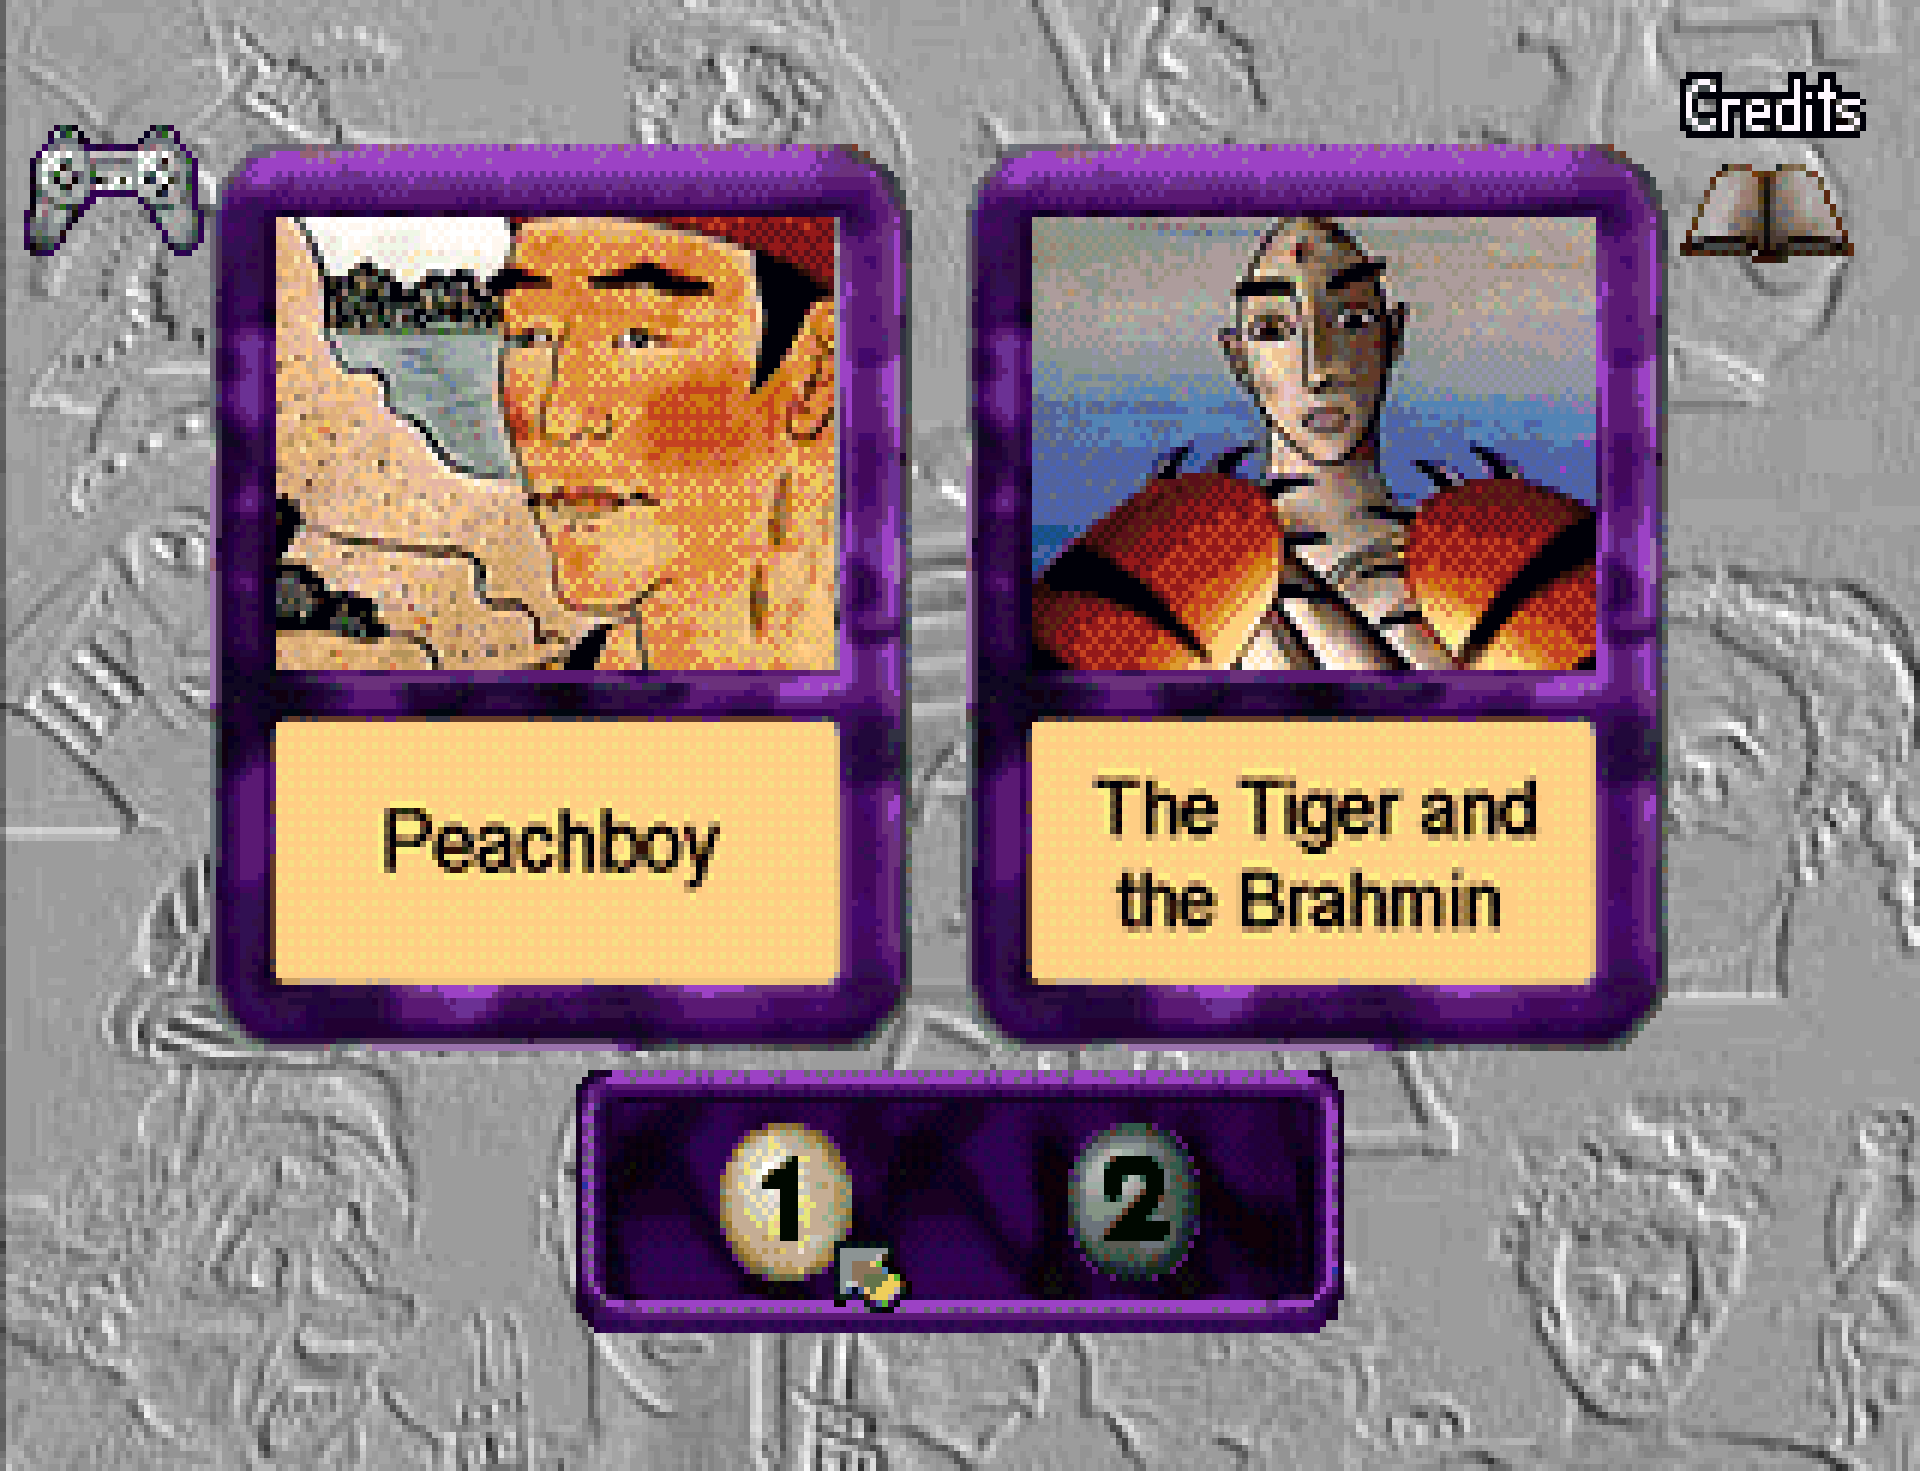
\includegraphics[width=\linewidth]{Games/StoryLaneTheater/Images/StoryLaneTheater5Image1.png}
        \caption{Story Lane Theater 5 - Screenshot 1}
    \end{subfigure}
    \begin{subfigure}{0.45\textwidth}
        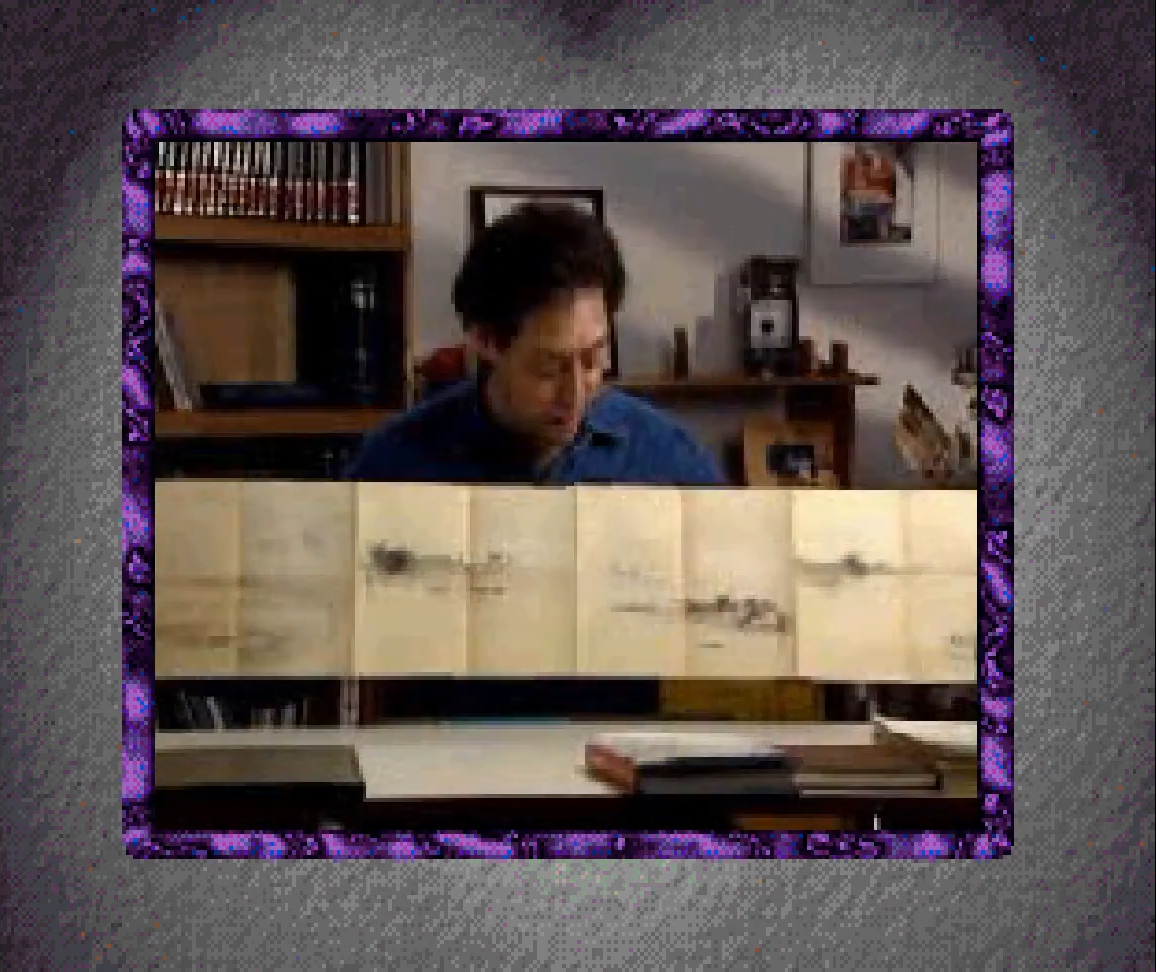
\includegraphics[width=\linewidth]{Games/StoryLaneTheater/Images/StoryLaneTheater5Image2.png}
        \caption{Story Lane Theater 5 - Screenshot 2}
    \end{subfigure}

    \begin{subfigure}{0.45\textwidth}
        \centering
        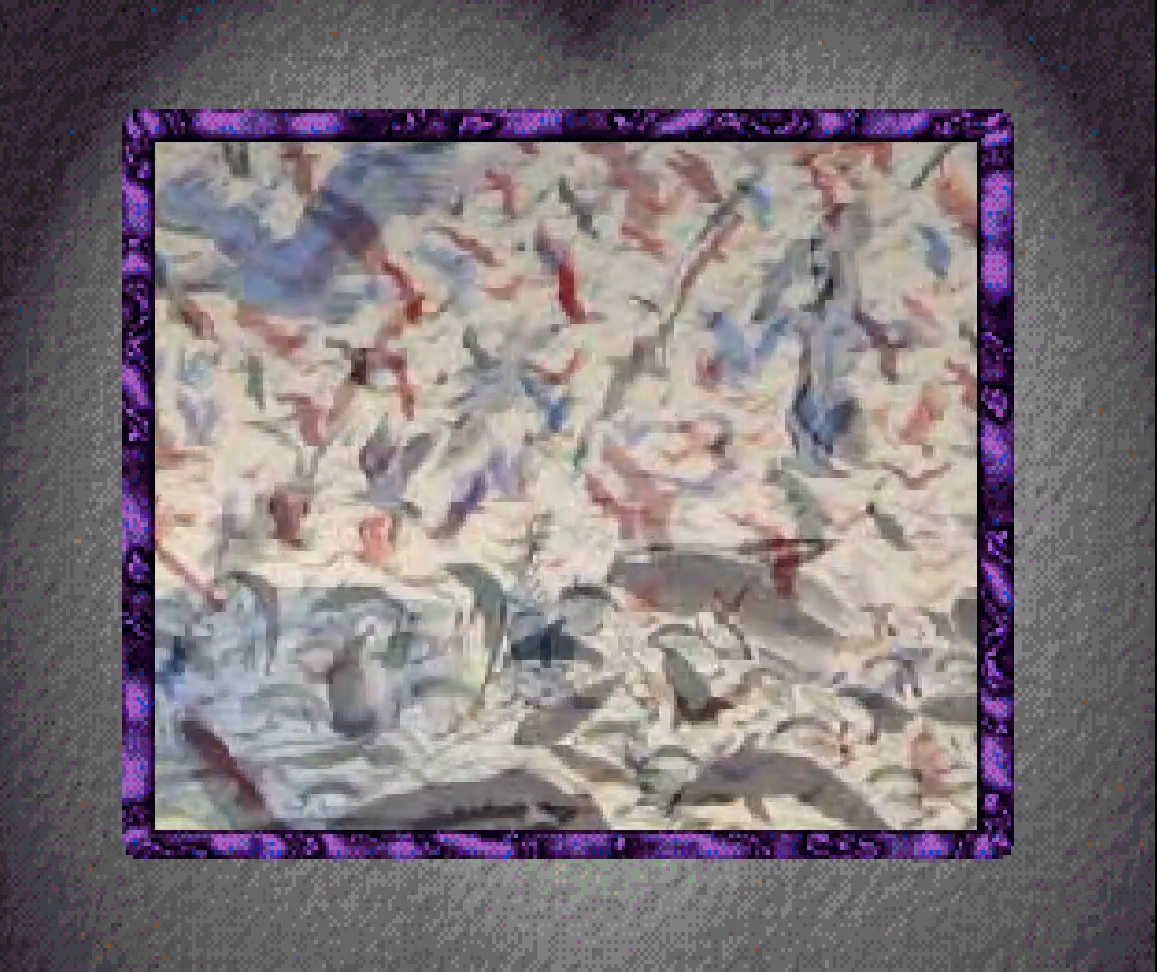
\includegraphics[width=\linewidth]{Games/StoryLaneTheater/Images/StoryLaneTheater5Image3.png}
        \caption{Story Lane Theater 5 - Screenshot 3}
    \end{subfigure}
    \begin{subfigure}{0.45\textwidth}
        \centering
        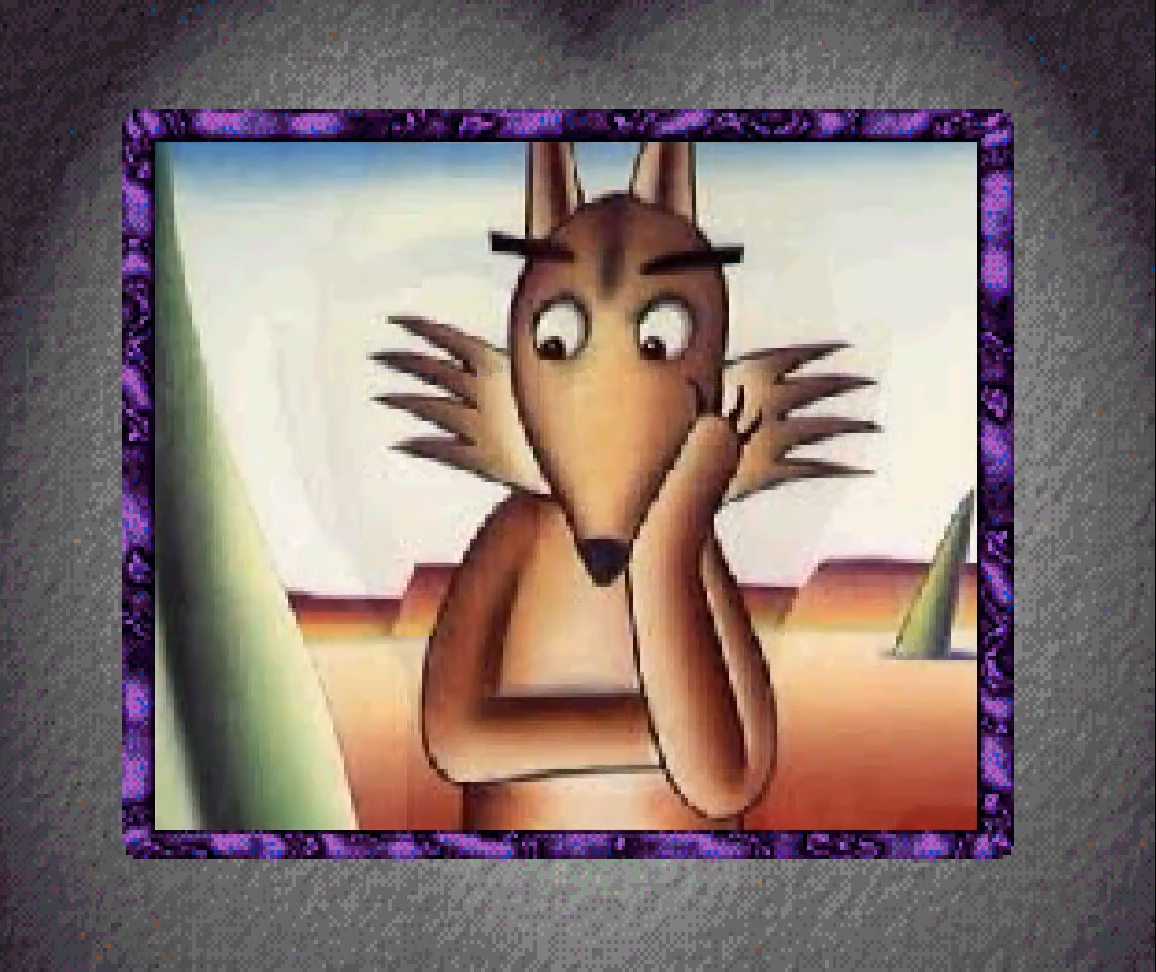
\includegraphics[width=\linewidth]{Games/StoryLaneTheater/Images/StoryLaneTheater5Image4.png}
        \caption{Story Lane Theater 5 - Screenshot 4}
    \end{subfigure}
    \caption{Screenshots from Story Lane Theater 5}
\end{figure}